\chapter*{Introduzione}
\addcontentsline{toc}{chapter}{Introduzione}

\section*{Obiettivi}
Gli argomenti del corso e i relativi esperimenti sono stati relativi a:
\begin{itemize}
    \item Programmazione di microcontrollori
    \item Gestione dei segnali analogici e conversione nel mondo digitale
    \item Manipolazione analogica dei segnali, amplificazione e sagomatura del segnale.
\end{itemize}

L'obiettivo ed esperimento finale è stata la costruzione di una catena per l'acquisizione del segnale generato da un SiPM e l'analisi di questo segnale.

\section*{Microcontrollore: NUCLEO-F429ZI}
Per lo svolgimento degli esperimenti è stata utilizzata una scheda di sviluppo NUCLEO-F429ZI.
La scheda ha al suo interno un microcontrollore STM32F429ZI, basato su architettura arm Cortex-M4 e con molteplici periferiche integrate come GPIO, ADC e Timer. Sono inoltre presenti sulla scheda un bottone, 3 LED e un debugger ST-Link, per permettere di flashare e debuggare la scheda senza utilizzo di hardware esterno.


\section*{Strumenti software}
\subsection*{STM32CubeMX}
STM32CubeMX è uno strumento fornito dalla STMicroelectronics per la configurazione iniziale del microcontrollore.

\begin{figure}[htb]
\centering
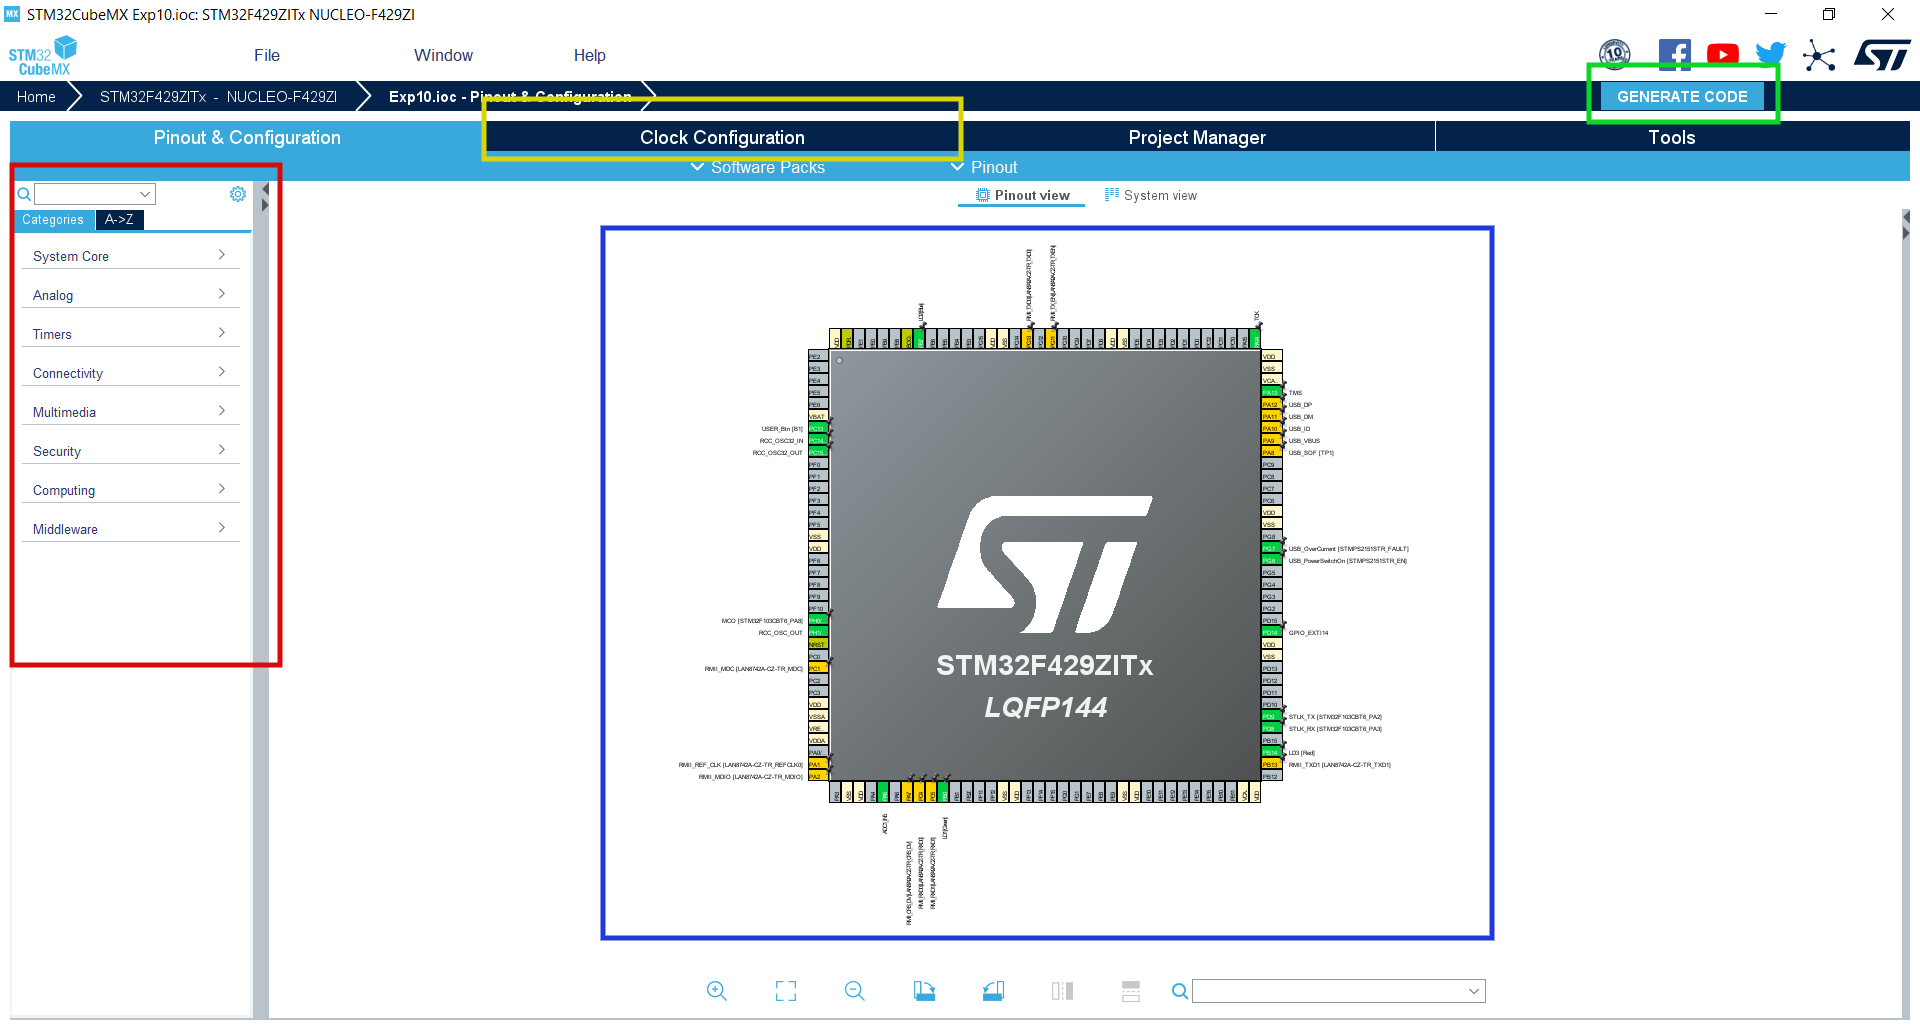
\includegraphics[width=\textwidth]{assets/introduzione/cube_mx_highlight.png}
\caption{Screen del software: in blu lo strumento per configurare i pin, in rosso la tab per configuare le periferiche, in giallo la tab per configurare il clock e in verde il tasto per generare il codice}
\end{figure}

Il software è scaricabile gratuitamente dal sito della ST\footnote{\href{https://www.st.com/en/development-tools/stm32cubemx.html}{https://www.st.com/en/development-tools/stm32cubemx.html}}.


Attraverso questo strumento è possibile, tramite una GUI, impostare la configurazione iniziale del microcontrollore: si possono inizializzare la le varie periferiche, assegnare funzioni ai pin, configurare i segnali di clock, abilitare gli interrupt, impostarne la priorità etc \dots

Una volta finito di configurare il tutto si può generare il codice e avere in output un progetto da utilizzare con Keil uVision.

\subsection*{Keil uVision}
Keil uVision è un IDE (Integrated Development Environment) di proprietà della arm. È possibile scaricarne una versione di prova attraverso il loro sito\footnote{\href{https://www2.keil.com/mdk5/uvision}{https://www2.keil.com/mdk5/uvision}}.
Usando questo strumento possiamo scrivere il codice, compilarlo, flashare il binario ottenuto sul microcontrollore. Inoltre ci permette di entrare in modalità \textit{debug}, nella quale possiamo inserire breakpoint all'interno del codice per mettere in pausa il codice, eseguire step by step le istruzioni e visualizzare il valore delle variabili e il contenuto dei registri in tempo reale, mentre il codice è in esecuzione.

\subsection*{MATLAB}
MATLAB è un ambiente di programmazione per l’analisi di dati, lo sviluppo di algoritmi e la creazione di modelli. 
Nel nostro caso è stato utilizzato per comunicare via seriale con il microcontrollore e per fare l'analisi e plot dei dati ricevuti da esso ricevuti.\footnote{\href{https://it.mathworks.com/products/matlab.html}{https://it.mathworks.com/products/matlab.html}}.